\section{Introduction}
VLIW processors allow for parallel execution of instructions thereby advancing instruction level parallelism. With the advent of $\rho$-vex it has become possible to reconfigure VLIW processors to suit the applications it's running. This is exactly the objective our group has been given and in this report we present our design that is optimized for the two benchmarks given, namely engine and fir.

\section{Benchmarks}
To optimize the VLIW processor for the given benchmarks a thorough examination of the benchmarks has been performed as has been described below.

\subsection{Engine}
The engine benchmark consists of a lot of divide operations as seen in figure \ref{fig:engine_call_graph}. The edge to rpm function is called 1742 times and amounts to 33.3\% of the execution time of the enginef function. The same thing can be said about the interpolate function. The edge to rpm function heavily depends on dividing as both the function itself and the fdiv\_func function execute divisions.Furthermore both the enginef and the interpolate function make use of division. This will therefore be an important factor in optimizing the processor. Further examination of the C code reveals that besides division, the interpolate function contains quite some if-else statements that usually get a member from a struct or perform a simple add or subtract operation.

\subsection{Fir}
The fir benchmark is concerned with the application of a fir filter. As revealed by the C code this involves calculating the sine, gaussian, and application of the fir filter. Figure \ref{fig:fir_call_graph} also reveals that there are some 64 bit add and subtraction operations. Besides those operations, round AndPackFloat64 is called relatively often. It is important to consider the extensive use of mathematical operations in our processor design.

\begin{figure}[ht!]
    %\centering
    \hspace*{-3.5cm}
    \begin{subfigure}{.65\textwidth}
    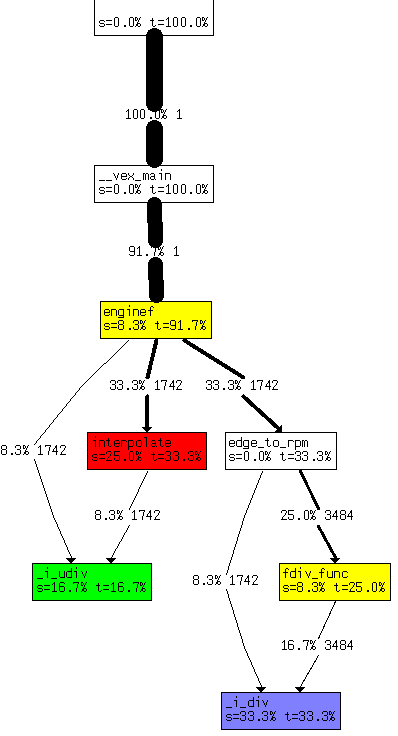
\includegraphics[scale = 0.75]{images/Engine-rgg.png}
    \subcaption{Engine: The call graph for the engine benchmark reveals that the benchmark performs a lot of divide operations (\_i\_div and \_i\_udiv).}
    \label{fig:engine_call_graph}
\end{subfigure}%
\begin{subfigure}{.5\textwidth}
  %\centering
      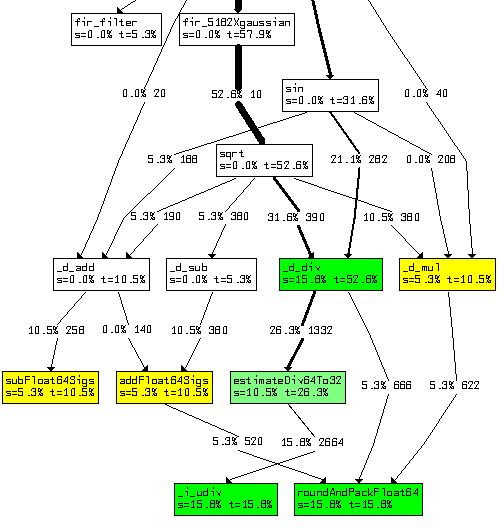
\includegraphics[scale = 0.8]{images/FIR-rgg3.png}
      \centering
    \subcaption{fir: The call graph for the fir benchmark reveals that the benchmark performs quite some divide operations (\_i\_udiv). Furthermore the add and subtraction operations, and the rounAndPackFloat are prominent.  Note that part of the graph is cut but that the nodes aren't relevant for show case of execution time as the relative execution time of those nodes (s) is zero.}
    \label{fig:fir_call_graph}
\end{subfigure}
\end{figure}
